\section{Iteration 1: Decomposition of the whole system}
\label{add:it1}

\npar In the first iteration, the whole system, ReMeS is decomposed. It takes
all the requirements and quality attribute scenarios as input.

\npar Two subsystems are recognized: a ``Remote Module Subsystem'' and the
``Portal''. This is shown in figure \ref{fig:add/it1/decomposition}.

\begin{figure}[H]
	\begin{centering}
		% TODO
		%\includegraphics[width=0.6\textwidth]{figs/decomposition/whole-system/decomposition.pdf}
		\caption{The subsystems of the ReMeS system}
		\label{fig:add/it1/decomposition}
	\end{centering}
\end{figure}

\subsection{Step 0: Confirm there is sufficient requirements information} 

% TODO de tekst in deze subsectie beschrijft niet helemaal wat in deze sectie
% moet komen. Ofwel schrappen we dit, ofwel maken we hier nog eens een overzicht
% van de requirements met prioritization door de opdrachtgever en invloed op de
% architectuur. 
% Referenced from: http://www.sei.cmu.edu/reports/06tr023.pdf

\subsection{Step 1: Identify candidate drivers}
\label{add:it1/drivers}

% TODO verwijs naar step 0?

\npar First of all when designing a decomposition for the whole system, the
choice of the drivers is very imortant since it will shape the architecture the
most. Therefore not only is the priority of the client for each quality
attribute scenario taken into account to choose the drivers, but also the impact of
that scenario on the architecure. These impacts are, together with the client
priorities, summarized in table \ref{table:add/it1/priorities}.

\begin{table}
	\begin{center}
		\begin{tabular}{| l | l | l | l | l | l | l | l | l | l |}
		\hline
		\textbf{Quality}			&	Av1	&	Av2	&	Av3	&	P1	&	P2	&	P3	&	M1	&	M2	&	M3	\\
		\hline
		\textbf{Client Priority}	&	H	&	M	&	L	&	H	&	M	&	M	&	H	&	L	&	M	\\
		\hline
		\textbf{Architecture Impact}&	L	&	L	&	L	&	H	&	H	&		&	M	&		&		\\
		\hline
		\end{tabular}
		\caption{An overview of all priorities which are takn into account when
		selecting the architectural drivers.}
		\label{table:add/it1/priorities}
	\end{center}
\end{table}

\npar Off course one wants to maximize the priority in both cases. Based on the
priorities in table \ref{table:add/it1/priorities}, one high priority and one medium
priority quality attribute scenarios are selected as architectural driver. An
overview of the selected drivers and their use cases is given below.

\begin{itemize}
  	\item P1 (High): Timely closure of valves
  	\begin{itemize}
  	  	\item UC8 (High) : send measurement
  		\item UC13 (High): Send alarm 
  	\end{itemize}
  	\item P2 (Medium) : Anomaly detection
  	\begin{itemize}
  	  \item UC10 (Medium) : Detect anomaly %TODO
  	\end{itemize} 
\end{itemize}

\npar The considered use cases includes the use cases listed below. 

\begin{itemize}
	\item UC7 (High): Send trame to remote device
	\item UC9 (High): Notify customer
	\item UC10 (Medium): Detect anomaly
\end{itemize}

\npar The choice of P1 is because it has the highest priority available (both a
high client priority and impact on the architecture). The reasons for selecting
P2 are more subtle since there are still combinations available (e.g. Av1) which
precede P2 in the prioriy hierarchy. The choice is twofold. First of all P2 is
very easy to combine with P1 because they both place constraints on the database
access in the two different operate modi (normal and overload). Second, 
%TODO waarom geen av1 of m1 ?

\npar Based on the architectural drivers, the remote module subsystem has to
provide functionality for remote module communication (receiving and sending
trames), trame storage, trame processing and customer communication. 

\npar In order to obtain a better understanding of the relationships between
these functionalities, a small domain model is drafted. Figure
\ref{fig:add/it1/draft} This model can then be refined later on
in this level of decomposition.

\begin{figure}[H]
	\begin{centering}
		% TODO
		%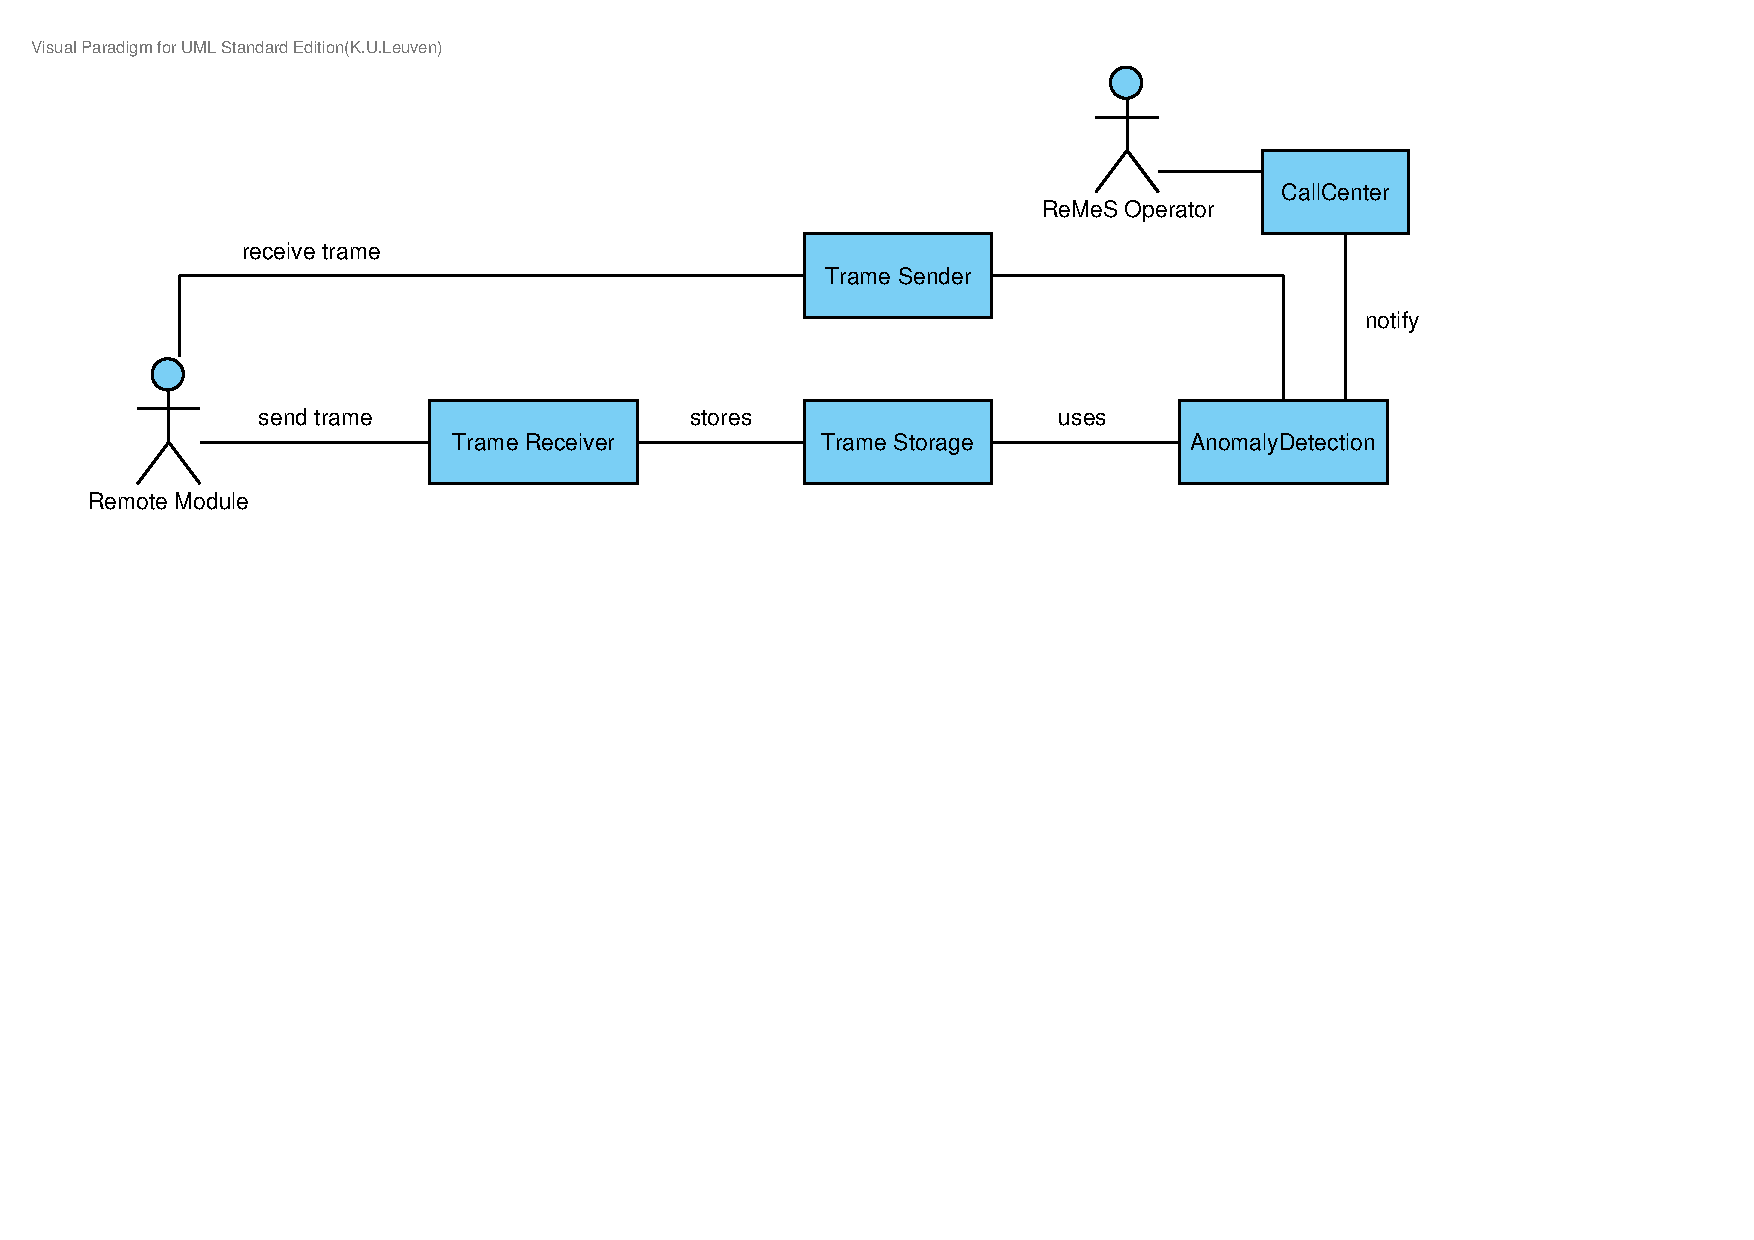
\includegraphics[width=0.6\textwidth]{figs/decomposition/whole-system/domainmodel-draft.pdf}
		\caption{Draft of the domain model used in the level 1 decomposition}
		\label{fig:add/it1/draft}
	\end{centering}
\end{figure}

\subsection{Step 2: Choose design concepts}
\label{add:it1/concepts}

\subsubsection{Tactics}
\label{add:it1/tactics}

% \paragraph{Availability} %TODO verplaatsen naar iteratie van storage.
% 
% \npar After selecting the drivers for the current decomposition, one has to
% choose the tactics to achieve them. Recall from section
% \ref{drivers:whole-system} that the first driver was Av1. All approaches to
% maintain availability involve either detection, recovery or prevention of
% faults.
% 
% \npar First of all, a fault needs to be detected. For this, there are three
% options: ping/echo, heartbeat and exceptions. It is important to notice that the
% latter is not very practical. This can be illustrated with a simple example.
% 
% \npar Suppose that a component $c_1$ depends on another component $c_2$. For
% some reason, $c_1$ does not need the services of $c_2$ for a duration longer
% than the detection interval of 5 seconds (see Av1). Within this time, no
% detection can occur, simply because there is no interaction between the
% components. For this reason, we eliminate exceptions as a primary fault
% detection system. However, exceptions will still have to be implemented in order
% to make the system fail gracefully (a component being unavailable will not
% cause the system to crash).
% 
% \npar Another detection method uses ping/echo. This primarily focusses on
% network connectivity and will not check the availabillity of the service itself.
% Again, this is not very practical. A server can be reachable, but the service on
% a certain port number may be unavailable. In this case, the ping/echo
% method would not detect the fault. 
% 
% \npar Heartbeat on the other hand, will be part of the system itself and will be
% able to check whether the service is still up and running. It will periodically
% (at most every 5 seconds) check the state of the system and send out a pulse
% to a heartbeat monitor if everything is runnning fine.
% 
% \npar Another advantage of using heartbeat is that the pulse can contain data,
% more specifically status data. For instance, a single failing disk in a RAID5
% array can cause a warning but will not cause the system to crash. This
% information can be included in the pulse of the heartbeat to inform the
% administrators to replace the failing disk.
% 
% \npar As a result, heartbeat seems the best solution to detect faults. 
% 
% \npar Detecting a fault is insufficient, resolving the fault is at least equally
% important. Once a fault has been detected, the faulting component must be taken
% out of action and be repaired or replaced with a working version. However, in
% order to guarantee an uptime of 99.9\%, there has to be a backup to take over in
% case of a component fault.
% 
% \npar As was the case in the previous paragraph, there are many alternatives.
% The most frequently used ones are active redundancy, passive redundancy and
% spare. The main criterion to select one of these is the downtime of the system.
% These downtimes are respectively in the order of miliseconds, seconds and
% minutes. An uptime of 99.9\% corresponds to 0.72 hours (= 43.2 minutes) of
% permitted downtime on a monthly basis. This number reveals potential problems
% when a spare is used because there can be only less the 10 failures a month. For
% this reason, use of spares is eliminated.
% 
% \npar The difference between active and passive replication is rather subtle.
% In an active replication scheme, the system will recover faster then in a
% passive replication scheme. However, all replicas should be in a consistent
% state. This increases the communication overhead, compared to a passive
% replication scheme. 
% 
% \npar On the other hand, the active replication scheme can also provide load
% balancing. If one replica has a higher load than another, the replica with the
% lowest load can be used to process the query. For this reason, the active
% replication scheme is selected. 

\paragraph{Performance} 

\npar For performance tactics there are three categories: resource
arbitration, resource management and resource demand.

\npar If there is more than one request to gain control over a resource, there
has to be some form of scheduling. By far the most used one is a priority
scheduler where request are served earlier when they have a higher priority.
This is particulary useful for alarms to still reach the appropriate parties in
time even when the system is in overload mode. 

\npar Secondly there is resource management. To process more than one trame at a
time, concurrency can be introduced. This can be done in various ways. Several
threads can be started on one processor, on separate processors or even on
separate systems. Another possibilitiy is off course increasing the available
hardware but since this is not a very cost effective solution, this is left out
of consideration.

\npar On a lower level one could also try to minimize network overhead by
only sending small amounts of data in each trame. This is achieved by
limiting the size of the trames to 160 bytes.

\npar To conclude a small overview is given of all selected tactics for this
decomposition.

\begin{itemize}
 	\item Av1 (High): Measurement database Failure
 	\begin{itemize}
 		\item Detection: Heartbeat 
 		\item Recovery : Active replication
 	\end{itemize}
  	\item P1 (High): Timely closure of valves
  	\begin{itemize}
  		\item Resource arbitration : Scheduling
		\item Resource management  : concurrency
		\item Resource demand      : limited tramesize
  	\end{itemize}
\end{itemize}

\subsubsection{Design Patterns}
\label{add:it1/patterns} %TODO verder uitwerken

\npar With respect to resource arbitration and resouce management, the
\emph{Active Object} design pattern is chosen for trame communication and
processing. Schedulers will determine the order in which trames are received,
processed and sent. These schedulers will have different scheduling policies,
implemented with the \emph{Strategy} design pattern, in order to allow operation
in different modes.

\npar The trames will have to be objectified. This will yield two advantages.
Firstly, the scheduler can be implemented using the \emph{Command Processor}
design pattern. Secondly, a unified language will exist for all vendor
specific trame formats.

%TODO verplaatsen naar storage.
% \npar To make the data highly available, the database will be replicated. This
% can be achieved by using the \emph{Replicated Component Group} design pattern.
% The database will be replaced with a front-end interface that replicates all
% requests to all the replicas. 

\npar To allow load balancing (and hence increase the performance) multiple
instances of the anomaly detection are created . This can be achieved by using
the \emph{Resource Pool} design pattern. 

%TODO: verplaatsen naar storage iteratie
To make this replication transparant to the users of the storage the
\emph{Business Delegate} is used.

\subsection{Step 3: Instantiate architectural elements and allocate responsibilities}
\label{add:it1/elements}

% TODO fig

\subsubsection{Communication unit}

\npar This module is responsible for all communication from and to remote
modules (all types of communication and both valves and control devices).
Incoming trames (from remote devices) are handed over to the storage scheduler.
Trames which need to be sent to to remote modules are dispatched to the correct
module through the correct medium.

\subsubsection{Storage Scheduler}

\npar This scheduler gets all incoming trames from remote modules and schedules
them for storage. Dependent on the active scheduling policy trames can be
prioritized over other trames. For instance, an incoming alarm trame for a gas
leak has top priority and has strict bounds on the delivery time (see the
quality attribute scenarios). Furthermore serves this scheduler as a buffer.
This is particularly useful when the storage unit is overloaded.

% \subsubsection{Heartbeat monitor cluster}
%  TODO: verplaatsen of weggooien.
% \npar The heartbeat monitor cluster is the result of the tactic to detect a
% fault, namely heartbeat. This component will monitor all other components to see
% if they are still alive (i.e. not crashed). Off course it is not unthinkable
% that the monitor component fails itself. Therefore this component has to monitor
% itself by for example an extra monitor that monitors the monitor.

\subsubsection{Storage of trames}

\npar This component is responsible for all storage of measuremnts (and
measurements only). It receives trames from the storage scheduler and notifies
the Anomaly Detection scheduler when a new trame is available.

%TODO: verplaatsen naar juiste iteratie
% \npar This component is the front end interface for database communication. This
% means that it communicates with all the instances of the physical storage to
% store a trame. Furthermore shall this unit notify the trame processing scheduler
% that a new trame entered the system. 

\subsubsection{Anomaly Detection Scheduler}

\npar When the storage unit has stored a new trame, this scheduler is notified
and fetches the freshly stored trame. Notice that this trame is not
the real, physical, trame that is stored in the datbase. One can think of it as
a kind of virtual trame, the actual trame will be fetched by the anomaly
detection unit. Analogous to the other scheduler this scheduler serves as a
buffer to prevent overloading on the anomaly detection unit. Once again
different scheduling policies can be switched on.

\subsubsection{Customer Communication Unit}

\npar This module is contacted by the anomaly detection. When the latter detects
an anomaly in the usage of one the utilities of a customer or a (non false)
alarm, then that customer (and possibly the emergency services) needs to
notified. This is the responsibility of the Customer Communication Unit.

\subsubsection{Anomaly Detection Instance Manager}

\npar The Anomaly Detection unit is responsible for running the algorithms to
discover anomalies. It receives virtual trames from the anomaly detection
scheduler so it can process them. After receiving such a virtual trame, the
real trame is fetched by sending a read query to the storage scheduler. Notice
that there are multiple instances of this anomaly detection unit. This allows
load balancing, cf. P2. 

\npar The task of this unit is the managing of all these instances. This
includes monitoring the load of all the instances, performing the read queries
and distributing the result (i.e. the trames). Upon detecting an anomaly two
possible actions (or both) can be undertaken. The first is sealing a valve if
it is a severe leak (this action is represented by the dependency between the
outgoing communication scheduler and the anomaly detection). The second is
notifying the approriate parties (the customer and/or the emergency services).

\subsubsection{Outgoing Communication Scheduler}

\npar The outgoing communication scheduler has as duty the scheduling of
trames which are sent to remote modules. There is a need for scheduling because
control trames to shut a valve need to reach the specified module in certain
time constraints according to P1. This scheduling can again be realized by the
use of different policies.

\subsubsection{Stakeholder Communication unit}

\npar This unit is responsible for all communication towards stakeholders (e.g.
customers, emergencyservices, etc.). 

\subsection{Step 4: Define interfaces for instantiated elements}
\label{add:it1/interfaces}

% TODO: fig

\npar All communication from and to remote modules goes through the remote
module communication unit. To support this behaviour this module offers a
\method{receiveTrame(\ldots)} method which is called by remote modules. Remote
modules in their part also offer a \method{receive(\ldots)} method which is called
by the communication unit upon sending a trame towards the the module. Components
who require a sending service (towards modules) can invoke the
\method{sendingTrame(\ldots)} method. Finally to allow the further processing of
incoming trames, a \method{scheduleForStorage(\ldots)} is needed where this
module can deliver incoming trames to.

\npar The storage scheduler offers two methods, namely
\method{scheduleForStorage(\ldots)} and \method{scheduleQuery(\ldots)}. The
former method acts as a registering point where trames can be delivered for
storage. The latter serves for the scheduling of components who want
to read the database. Furthermore does this component requires one method
\method{storeTrame(\ldots)} to permanently store a trame in storage.

\npar To permanently store trames the storage component was introduced. Storage
offes one method \method{storeTrame(\ldots)} to realize this functionality.
Thereupon is the anomaly detection scheduler notified that a new trame is
available for processing. Therefore the scheduler has to offer a
\method{notify(\ldots)}, which can be called by the storage component.

\npar As said in the previous section the anomaly detection schedulers offers a
\method{notify(\ldots)}, where the storage component can notify this scheduler
when a new trame is ready for processing. Upon receiving a notification this
scheduler can schedule this trame for processing. Afterwards the (virtual)
trame is sent towards the anomaly detection unit for processing using the
\method{processTrame(\ldots)} method.

%TODO: replicas
\npar The anomaly detection unit fetches the trames by performing a read query
and sending it to the storage scheduler. The scheduler therefore has a
\method{scheduleQuery(\ldots)} which return the (real) trame. When the trame is
returned this unit can process it. To seal a valve a trame can be constructed to
send to the remote module (i.e. valve), therefore the outgoing
communication scheduler offers the \method{scheduleForSend(\ldots)} method. The
notification of third parties (i.e. emergency services, customers) can be done
through invocation of \method{notify(\ldots)}.

\npar The stakeholder notification unit offers one method
\method{notifyThirdParty(\ldots)} which is to be invoked by any component who
wishes to notify e.g. the emergency services and/or one or more customers. These
third parties have to offer in their part a \method{receive(\ldots)} method.

\subsection{Step 5: Verify and refine}
\label{add:it1/verification}

\npar In this step, we verify that that the element decomposition thus far meets
the functional requirements and quality attribute requirements. Also, child
elements are prepared for further decomposition.

\npar Three things have to be verified. First, we will verify that all
functional requirements and quality attribute requirements of the parent element
have been allocated to one or more child elements in the decomposition.
Secondly, all responsibilities that were assigned to child modules are
translated into functional requirements for the individual items and finally,
quality attribute scenarios for individual child elements are refined if
necessary.

\npar We will list all the child elements, together with their allocated use
cases and quality attribute requirements. If a requirement is split or
delegated, it is also mentioned in the list. To conclude an overview is given of
resolved requirements in this iteration.

\begin{itemize}
	\item Communication Unit
	\begin{itemize}
	  	\item UCx : Retrieve Customer from remote module identification %TODO dit
	  	% wordt toegewezen aan communication unit, maar het is wel een oproep van
	  	% een methode op other (``getCustomerby etc)
	  	\item UCy : Retrieve Remote Module protocol
		\item UC7': Send trame to remote device (split)
		\item Av2': Missing measurements (split)
		\item M1' : Dynamic pricing (split)
		\item M3' : Decentralized electricity generation (split)
	\end{itemize}
	\item Storage Scheduler
	\begin{itemize}
		\item P1' : Timely closure of valves (split)
	\end{itemize}
	\item Storage
	\begin{itemize}
		\item Av1 : Measurement database failure (delegated)
		\item Av2' : Missing measurements (split)
	  	\item P3': Requests to the measurement database (delegated)
	\end{itemize}
	\item Anomaly Detection Scheduler
	\begin{itemize}
		\item UCz: Determine the operational mode (derived)
		\item P1' : Timely closure of valves (split)
	  	\item P2': Anomaly Detection (split)
	\end{itemize}
	\item Anomaly Detection
	\item Customer Communication Unit
	\begin{itemize}
		\item UC9: Notify Customer
	\end{itemize}
	\item Outgoing Communication Scheduler
	\begin{itemize}
	  \item P1' : Timely closure of valves
	\end{itemize}
	\item Other functionality
	\begin{itemize}
	  	\item UC1: Log in
	  	\item UC2: Log off
	  	\item UC3: Register customer
	  	\item UC4: Unregister customer
	  	\item UC5: Associate device to customer
	  	\item UC6: Customize customer profile
	  	\item UC11: Operate remote actuator remotely
	  	\item UC12: Set alarm recipients
	  	\item UC14: Request consumption predictions
	  	\item UC15: Generate invoice
	  	\item UC16: Mark invoice paid
	  	\item UC17: Perform research
	  	\item Av3: Third Party Billing Service failure
	  	\item M1': Dynamic pricing
	  	\item M2: Fine-grained metering for enterprises
	  	\item M3': Decentralized electricity generation
	\end{itemize}
	\item Resolved requirements
	\begin{itemize}
		\item UC7': Send trame to remote device (split)
		\item UC8 : Send measurement
		\item UC13: Send alarm
		\item UC10: Detect anomaly
		\item P1' : Timely closure of valves (split)
		\item P2' : Anomaly detection (split)
	\end{itemize}
	\item 
\end{itemize}
